\section{Password Protection}
\label{passwordprotection}
In almost all systems, users are able to choose and update their passwords. However, they
may sacrifice password security for usability since a long and random secure password is
less memorable.
As user passwords are easier to be compromised when their personal
information is available to the attacker, we investigate how users
can protect their passwords against such attacks.
%However, people are bothered to remember secure passwords because the
%usability of secure passwords is low.
%Considering the trade-off between password usability and password
%security, we seek to make passwords more secure while maintain
%acceptable memorability.


%\subsection{Distortion Function}
To increase the password security while retaining good memorability, we introduce
the {\em Distortion Function}, which performs a transformation on user
passwords. A distortion function converts user passwords to more
secure strings by either breaking password semantics or increasing
password entropy. Therefore, the user only needs to remember the
original password and apply a simple function on it to create a stronger
password. This distortion function can be chosen by users so it could
be either linear or non-linear.

We conducted a proof-of-concept study to show the effectiveness of
distortion function on password security. In our study, we propose two
types of distortion functions. 
%
The first type of distortion function maps each password character to
another character. For instance, {\em $add_1$} function simply replaces
each letter with the one 1 letter later in the alphabet and replaces
single digital number $i$ with $(i+1) mod 10$. It is similar to the
Caesar Cipher~\cite{kaufman-textbook}. In another example, {\em $add_pi$}
is a non-linear function that replaces characters by the position
specified by $\pi$, which is $314159 \ldots$. It replaces the first
letter with the one 3 letters later and the second letter with the one
1 letter later, etc.
%
The second type of distortion function adds an extra fixed character
between any pair of characters in passwords. The length of passwords
become twice of the original password minus 1 when the length is
larger than 1. We call this distortion function {\em $gap_x$}, in which
``x" represents the extra symbol. For example, when $x = ``a"$, Alice's
password ``alice816" will be extended to ``aalaiacaea8a1a6" after the
distortion function. 
%In our study, we choose "gap0", "gapa", and "gap!".

The distortion function must be simple enough for users to remember
and generate the passwords. We apply a number of distortion functions
on each of the password in 12306 dataset individually and calculate
the Coverage for the converted passwords.  As Figure~\ref{f4} shows,
the distortion functions are effective on increasing password
security by greatly reducing the
correlation between user passwords and personal information.
%
Moreover, we notice that the impacts of various distortion functions
are also different. For example, {\em $add_!$} performs the best
(Coverage is 0 for all users so it is not shown in Figure~\ref{f4}) since users rarely have special
characters in their personal information. Surprisingly, the non-linear
{\em $add_pi$} function does not produce a better result than other
linear functions such as {\em $add_1$} because digits preferred by Chinese
users are more likely to have coincidence wrong matches due to its low entropy.
%However, these coincidence matches tend to be short in length, so its
%Coverage won't increase too much as we stress continuation in match
%when computing Coverage.
 \begin{figure}[t]
\centering
  \caption{Coverage distribution.}{}
  \label{f4}
    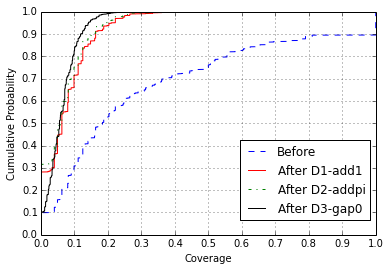
\includegraphics[width=0.4\textwidth]{fig/dist2}
\vspace{-0.1in}
\end{figure}

We conclude that distortion functions can mitigate the problem of
including personal information in user passwords without sacrificing
password usability.  Moreover, distortion function is also a cure for
semantics-aware password cracking methods~\cite{veras2014semantic},
which leverages semantic patterns in passwords to crack other
passwords. After applying a distortion function, the semantic pattern
is no longer available. Besides, distortion function is effective against PCFG
~\cite{weir2009password}, since it generates unrecognizable letter segments, which are not likely to be covered in commonly-used password
dictionaries.

The main weakness of distortion function is that it has to be kept
secret. If an attacker knows the distortion function used by a user,
cracking the user's password is as easy as cracking a plain
password. However, as users are able to choose their own distortion
functions, due to the large pool of potential distortion functions, it
is hard for attackers to guess which one is used or test all popular
distortion functions. Similar to the functionality of adding salt to
password, distortion functions make it harder to perform off-line
brute-force attack on a large password dataset. This is because
distortion functions make the passwords in the dataset sparser and
more unpredictable. 
 




